\chapter{Analýza}
V této kapitole bude probrána specifikace a požadavky na API a požadavky na celkové fungování hry.
Taktéž bude zde probrána analýza již existujících herních API.

Cílem této práce je vytvořit zdokumentované jednotné API které bude jak pro samotné hraní hry tak i pro backoffice.
\section{Analýza již existujících herních API}
V této části se představí dvě již existující online hry s postupem který se ukládá. Těchto her ovšem není mnoho. Většina online her co jsou na webu je bez přihlašování a také bez postupu či evoluce. Takovéto prémiové hry bývají většinou jako desktopové aplikace a bohužel zde by se špatně analyzovala odcházející a přicházející komunikace.
Ovšem byla mi doporučena jedna hra, která je vytvořená přímo pro hraní za pomocí API.\subsectionref{sub:SpaceTraders}

\subsection{SpaceTraders API}\label{sub:SpaceTraders}
SpaceTraders je hra založená na REST API kde se může kontrolovat a získávat flotily vesmírných lodí a za jejich pomocí objevovat, obchodovat a vybojovat si vlastní cestu skrz galaxii. Hra je určena k vytvoření si vlastního frontendu a nebo k automatizaci přes jakýkoli jazyk jakožto API na kterém se dá hezky naučit nový jazyk. API je zdokumentováno za pomocí OpenAPI a Stoplight jako zobrazovací rozhraní. \cite[]{spacetraders}

Pro dotazování využívají jak parametrů dotazu tak proměnných v dotazované URL\@.

Token se vkládá do hlavičky ve formátu \texttt{'Authorization: Bearer INSERT\_TOKEN\_HERE'}. Tento token je ve formátu zakódovaného JWT \sectionref{sec:jwt} objektu pomocí RS256.
Můžeme ho vidět dekodovaný na obrázku \ref{fig:jwt_spacetraders}

\begin{figure}[!ht]
    \centering
    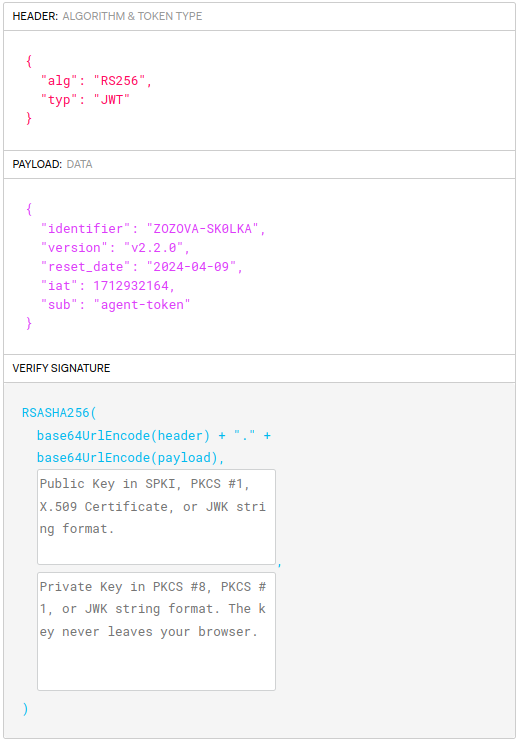
\includegraphics[width=0.5\textwidth]{figures/spaceTraders/jwt.png}
    \caption{Dekódovaný token ze hry SpaceTraders pomocí dekoderu.\cite[JWT decoder]{jwt_decoder}}
    \label{fig:jwt_spacetraders}
\end{figure}

Hra jako první vyžaduje registraci přes endpoint \texttt{/v2/register}. Ten vrátí údaje o novém agentovi spolu s autentizačním tokenem \coderef{code:space_login}[řádek 3]  se kterým se dále bude ověřovat ve všech dalších požadavcích.

\begin{listing}[!ht]
    \inputminted[breaklines]{json}{resources/code/spaceTraders/login.jsonc}
    \caption{Odpověď na požadavek na registraci \protect\footnotemark }
    \label{code:space_login}
\end{listing}
\footnotetext{Velká část dat musela být pro přehlednost smazána}

Jako odpověď používají formát JSON, kde mají vždy objekt \texttt{data} jako objekt zájmu a poté dodatečné objekty jako třeba \texttt{meta} ve kterých může být například stránkování. % TODO odkaz na stránkování
Status odpovědí používají v rámci nepsaných pravidel % TODO odkaz na ty pravidla někde v restku
a dále v obsahu rozšiřují co přesně je na daném požadavku špatně. \coderef{code:space_error}


\begin{listing}[ht!]
    \inputminted[breaklines]{json}{resources/code/spaceTraders/error_response.jsonc}
    \caption{Výpis chyby při požadavku odletět na jinou planetu. (Loď je aktuálně na planetě a není na orbitě. Loď před odletem na jinou planetu musí být na orbitě)}
    \label{code:space_error}
\end{listing}

\section{Specifikace požadavků}
Pomocí analýzy her a vyčlenění požadavků na funkcionality hry od ostatních členů týmu a za pomocí analýzy dostupných nástrojů pro tvorbu API byly vytyčeny požadavky a funkce co by mělo API podporovat. API by mělo podporovat CRUD operace se základními objekty, jejich filtrování, stránkování, a lazy load. API by taktéž mělo podporovat přihlašování a kontrolu před základními typy útoků jako je SQL injection, DDOS a DOS útok a neoprávněný přístup díky chybám v API.

Taktéž by mělo podporovat validaci všech vstupních dat (rozsahy vstupních hodnot, nepovolovat speciální znaky, kontrolovat správný postup operací při hraní hry) a mělo by mít koncové body pro samotné hraní hry.

\subsection{Funkční požadavky}
Nyní si představíme funkční požadavky na API od ostatních členů týmu. Tyto požadavky se měnily a rozšiřovaly postupně s průběhem návrhu i implementace. Některé požadavky, které vyšly primárně z backoffice se využívají ve frontendu případně naopak.

\subsubsection*{Požadavky které byly vyčleněny primárně z backoffice sekce.}

\begin{enumerate}[label=\textbf{F\arabic*}:, leftmargin=*, align=left]
    \item \textbf{CRUD operace} Nad základními objekty se kterými se počítá že se bude často pracoavat a upravovat pomocí enpointů. Těmito objekty jsou \texttt{akce, efekty, předměty, charaktery a jejich vlastnosti, dobrodružství, kampaň, obchody, nepřátelé, překážky, lokace, části lokace}
    \item \textbf{Filtrování} Možnost vyhledat objekty podle vstupních parametrů u koncových bodů které poskytují seznam objektů.
    \item \textbf{Lazy load} Způsob jakým se načítají data. Tato funkcionalita umožňuje vracet pouze daný objekt bez jeho závislostí a nebo může vrátit jen závislosti, které se určí. Výsledkem je rychlejší zpracování a menší objem dat, když nás nezajímají závislosti objektu ale pouze objekt samotný. Namísto objektu se vrátí identifikátor daného objektu.
    \item \textbf{Stránkování} Možnost rozdělit data na více částí. Tato funkcionalita umožní postupné zpracování dat a kratší časy potřebné k vyhodnocení jak v API tak ve zobrazovací části.
    \item \textbf{Caching} Již jednou zpracovaná data z databáze není třeba znovu získávat z databáze pokud nedošlo ke změně. Tato funkcionalita umožní násobně rychlejší odezvu pro opakované získávání stejných dat.
    \item \textbf{Administrátorská práva} Ne všichni mohou mít přístup pro úpravu dat v databázi. Díky administrátorským přihlašovacím údajům a následnému tokenu se budou moci upravovat a vkládat data do databáze.
    \item \textbf{Validace} Data vkládaná do databáze budou validována a případně vrátí popisující chybovou hlášku podle které půjde snadno identifikovat chybu vstupních dat a následně ji opravit.
\end{enumerate}

\subsubsection*{Požadavky primárně ze strany zobrazování a hry.}


\begin{enumerate}[label=\textbf{F\arabic*}:, leftmargin=*, align=left]
    \item \textbf{Získávání objektů} Bude umožněno získávat jakékoliv objekty z databáze které neobsahují herní data či jiné citlivé informace.
    \item \textbf{Podpora herního průběhu} Uživatel bude moci projít celým encounterem a interagovat s věcmi v něm za pomocí řady validovaných přehledně uspořádaných koncových bodů.
    \item \textbf{Zamezení zneužití} Postup operací v herním průběhu bude kontrolován aby se zamezilo případným zneužitím nebo obcházením pravidel hry.
    \item \textbf{Přihlášení} Uživatel se bude moci přihlásit a získat token pro ověření v dalších požadavcích.
    \item \textbf{Herní data} Uživatel bude mít pod svým účtem uložený postup hry a bude moci pokračovat tam kde skončil. Stejně tak bude mít možnost vytvářet nové postavy pro kampaně a bude moci vytvářet nové dobrodružství.
    \item \textbf{Validace} Obsah vstupních dat bude validován a případě vrátí smysluplnou chybovou hlášku.
    \item \textbf{Obrázky} Bude možné získat obrázek z url adresy přiložené k objektu. Případně bude možné měnit jeho velikost.
\end{enumerate}



\subsection{Nefunkční požadavky}
Nyní si vyhradíme nefunkční požadavky. Tyto požadavky vznikaly stejně jako požadavky funkční. Tedy postupně s vývojem od všech členů týmu.


\begin{enumerate}[label=\textbf{F\arabic*}:, leftmargin=*, align=left]
    \item \textbf{Rozdělení API na dvě části} Logické rozdělení API na dvě části, protože nechtěli jsme mít dva různé projekty na mapování dat z databáze a samotné hraní hry. Proto bylo rozhodnuto že herní logika i mapování bude v jednom projektu a k tomu jsme museli přizpůsobit i naši spolupráci a podpůrné technologie.
    \item \textbf{Dokumentace} API bude zdokumentováno za pomocí OpenAPI a Swagger jako zobrazovací rozhraní koncových bodů. Zároveň poslouží jako skvělé ladící rozhraní.
    \item \textbf{Hosting} API stejně jako ostatní části budou hostovány na veřejných serverech.
    \item \textbf{Přehlednost} Koncové body API by měly být samopopisující a neměly by jít špatně použít.
    \item \textbf{Standardizovanost} API se bude držet ověřených dobrých praktik z praxe a udržovat jednotnost a standardizovanost.
\end{enumerate}

